\chapter{NDVI-MAP FUNCTIONS AND USER GUIDE}
\label{chap:tibet}

\section{What can app do?}

Application can enable you to envision \gls{ndvi} mean information for any date accessible in the database. It likewise gives the usefulness of sending out the information into \gls{csv} record and messaging it to whosoever you need. \\
It likewise causes you visualize information utilizing diverse levels - Country wise, State wise and District.

\section{A user guide/manual}

\subsection{Getting Started}

\begin{itemize}
    \item \textbf{Downloading the app} \\ 
    Right now, the app is in process of being submitted to App Store for review. Once it is approved by Apple, you can utilize the "EyesOnCrops" application by downloading it from the Apple Store. 
    
    \begin{itemize}
        \item Open the App Store and type "EyesOnCrops" in search bar.
        \item Download and introduce the "EyesOnCrops" application on your gadget.
        \item Once the app is downloaded and installed, it will look like this on your device. You can have a look at Fig 2.1 for your reference.
        
        \begin{figure}[H]
            \centering
            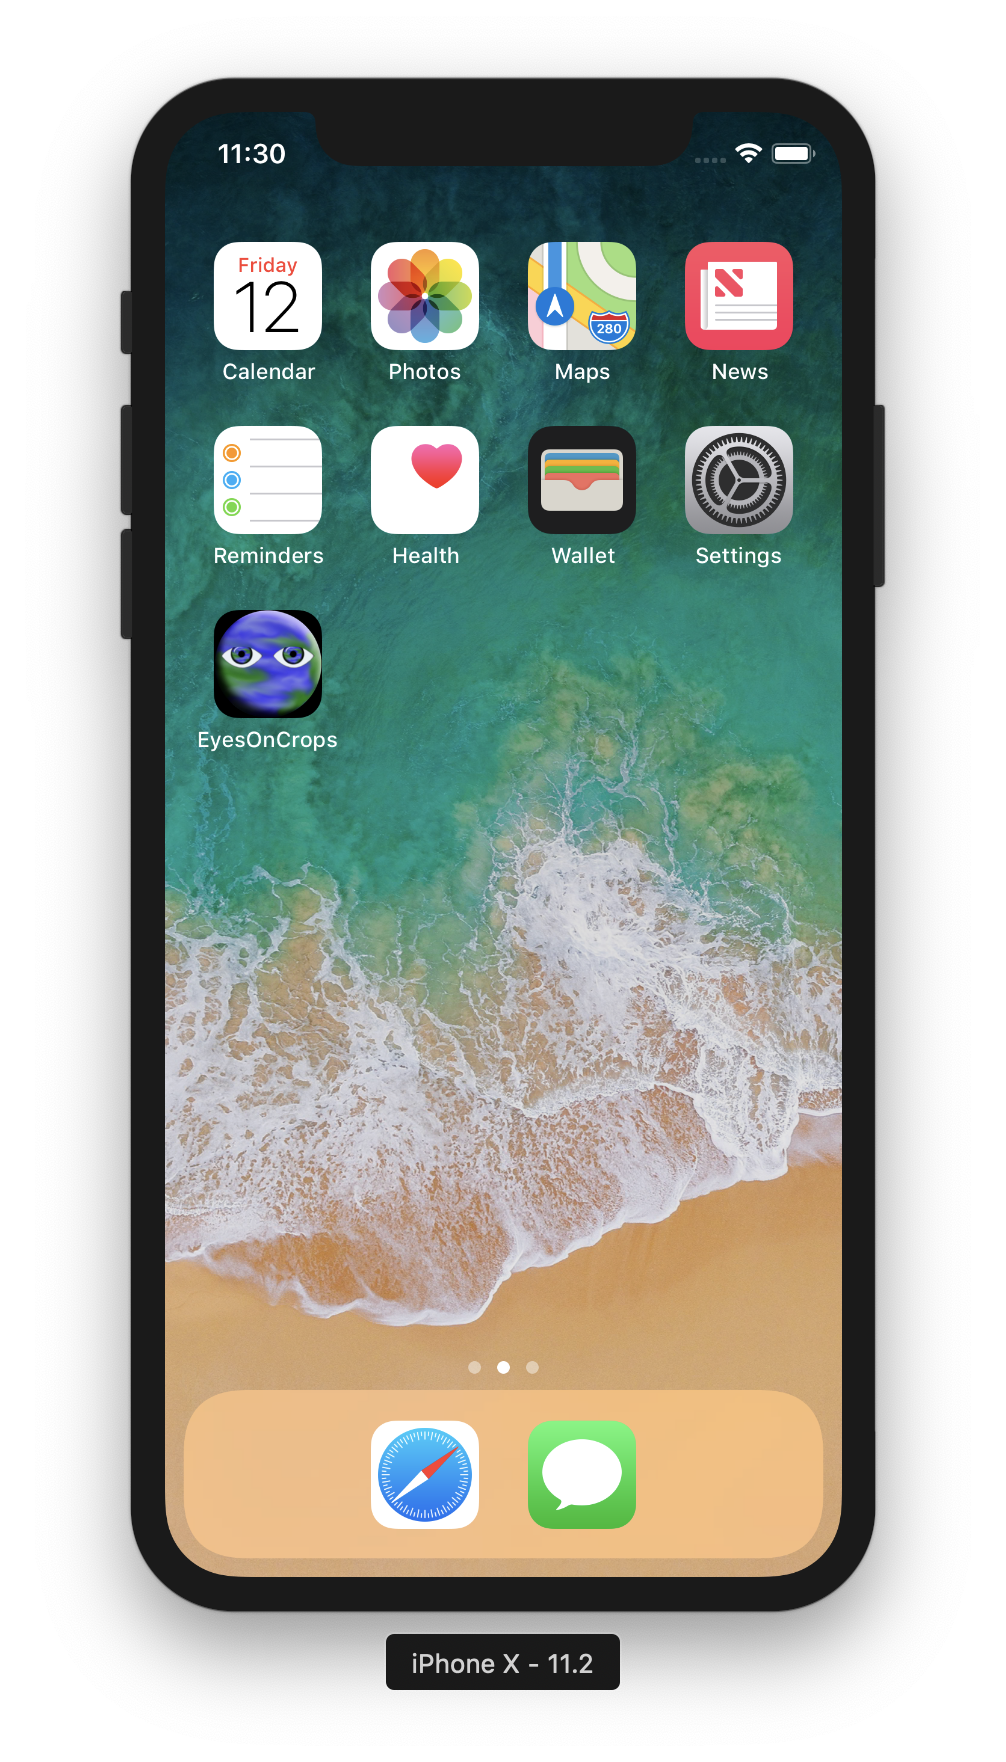
\includegraphics[width=0.5\linewidth]{figures/ch2/app_icon_screen.png}
            \caption{\label{fig:app_icon_screen} iPhone screen after downloading the app}
        \end{figure}
    \end{itemize}
    
    \item \textbf{Sign in} \\
    By tapping on app icon on fig 2.1, it will lake you to landing screen of the app which is also called as main screen.
    
     This screen gives you two options, which are (as shown in fig 2.2) :
     
       \begin{figure}[H]
            \centering
            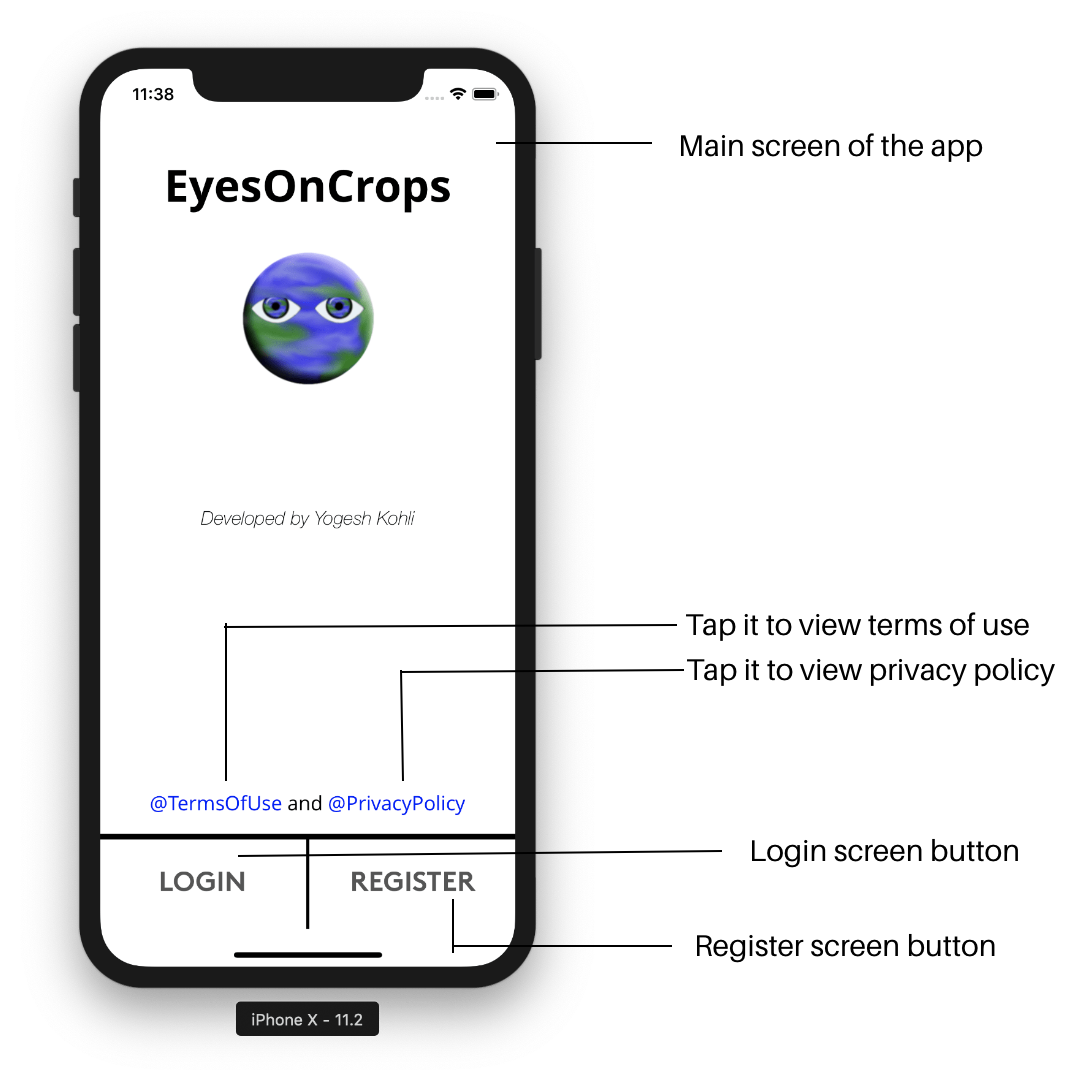
\includegraphics[width=0.5\linewidth]{figures/ch2/main_screen.png}
            \caption{\label{fig:main_screen} Main / Landing screen of the app}
        \end{figure}

    \textbf{1. Login} \\
    \textbf{2. Register via Email} \\
    
    If you select Login, it takes you two that screen which gives you options to enter the app. It has shown in fig 2.3.
    
    \begin{figure}[H]
            \centering
            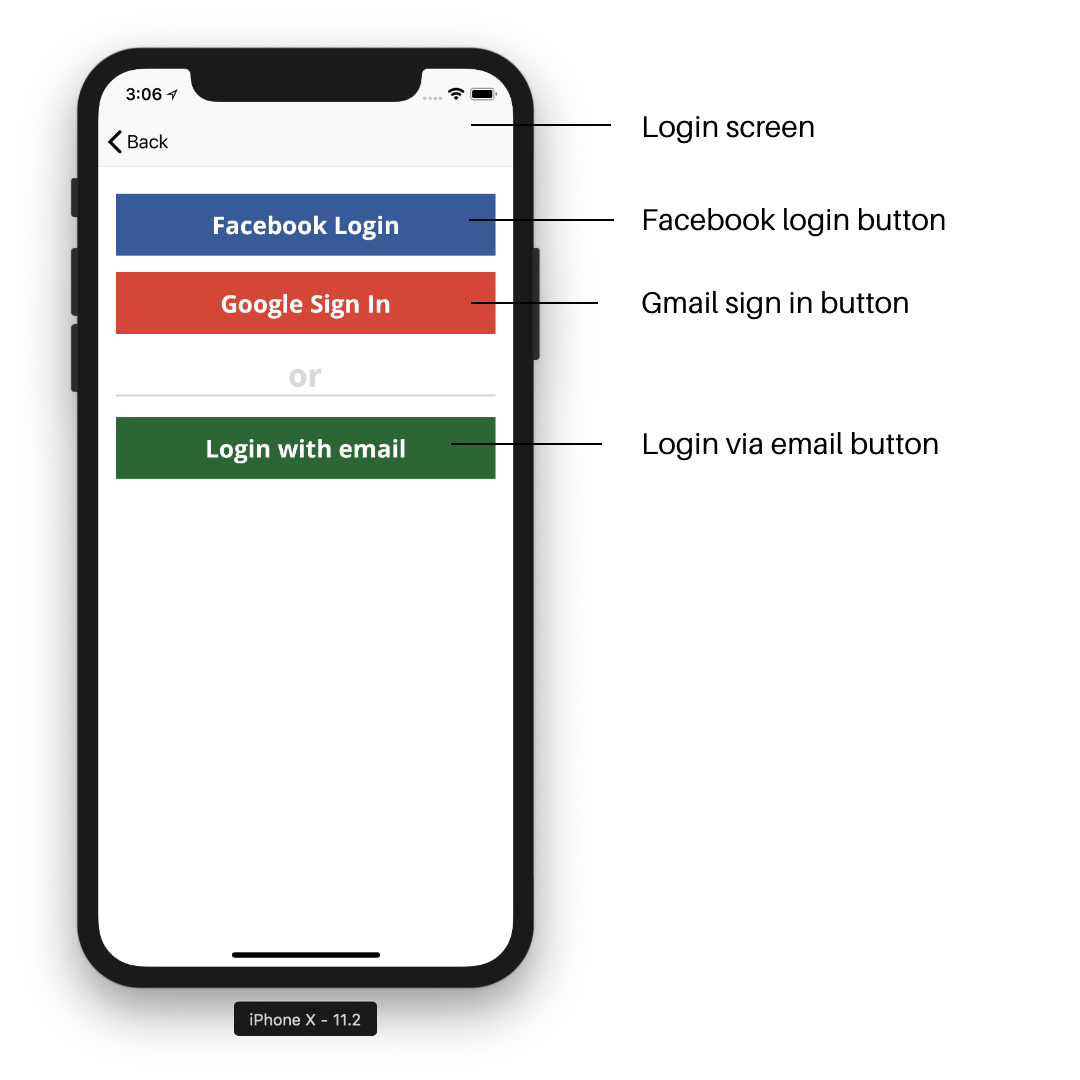
\includegraphics[width=0.5\linewidth]{figures/ch2/loginOptions.png}
            \caption{\label{fig:main_screen} Login options in the app}
    \end{figure}
    
     \textbf{1. Sign in via Social Accounts}
     
     \begin{itemize}
         \item Facebook login
         \item Gmail login
     \end{itemize}
   
     \textbf{2. Sign in via Email} \\
     
     Now, that you have decided to login via email option, it takes you to that screen which requires your credentials to enter the app, by entering the right credentials and pressing login button, you enters the app. The screen has shown in the fig 2.4.
     
     \begin{figure}[H]
            \centering
            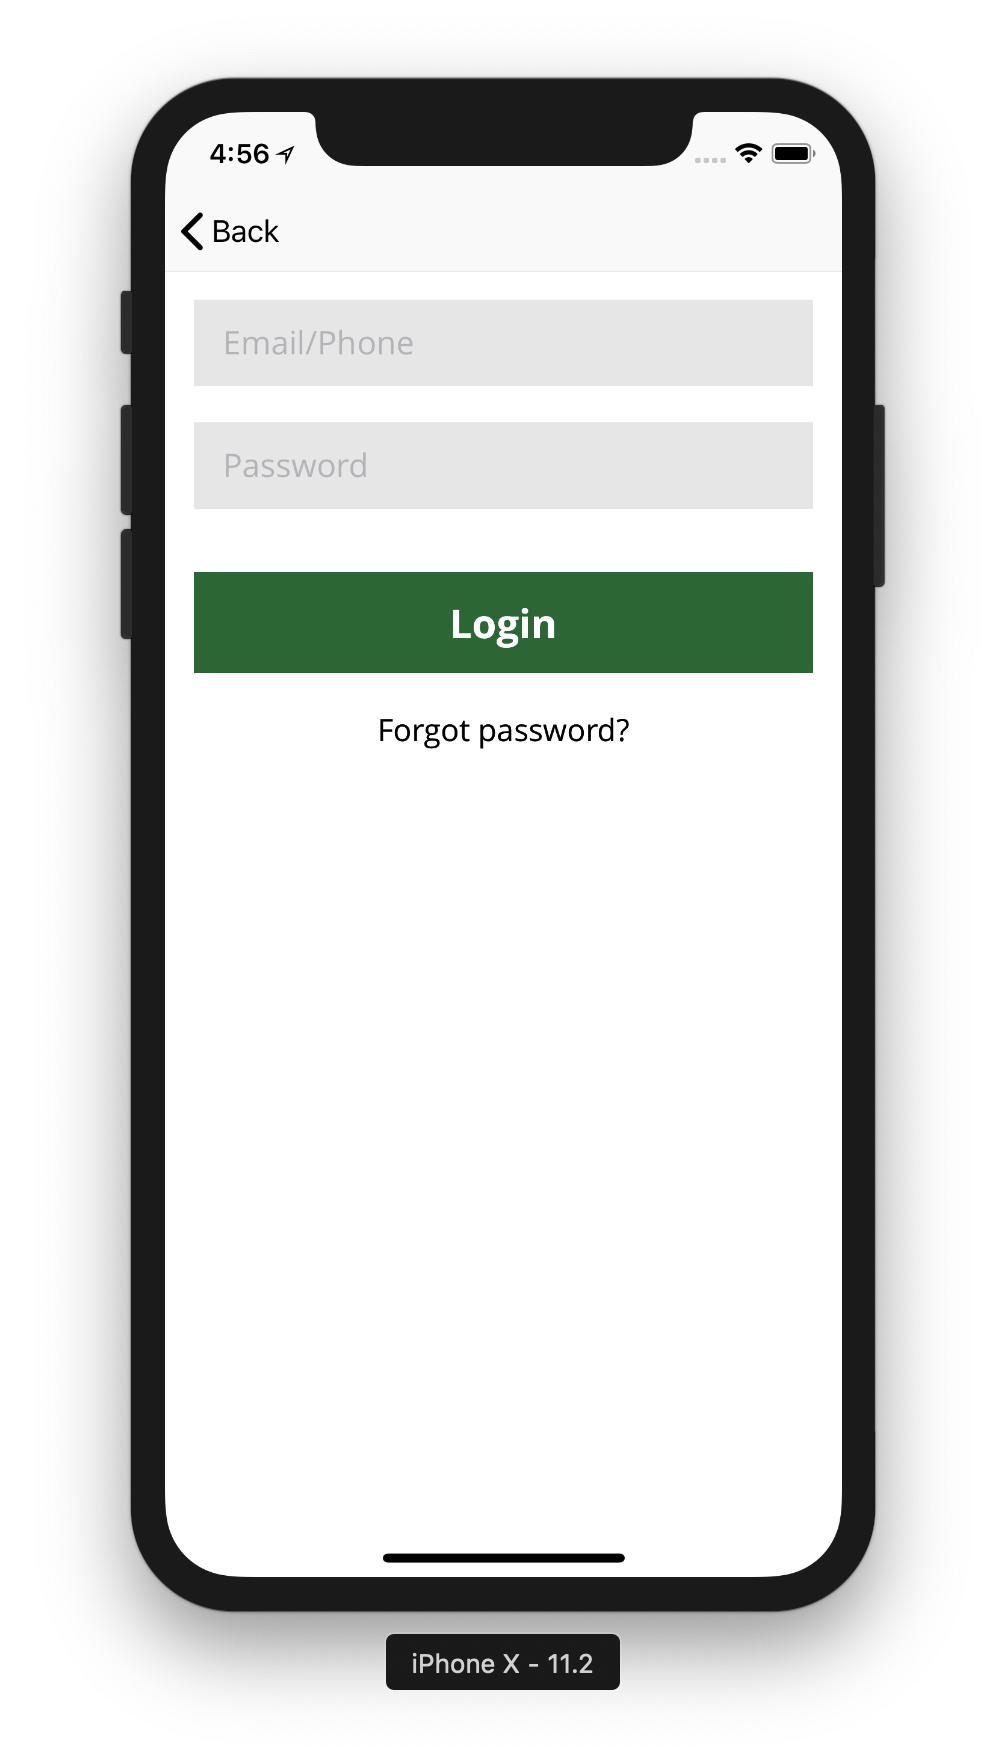
\includegraphics[width=0.5\linewidth]{figures/ch2/login_email.png}
            \caption{\label{fig:main_screen} Login via email}
    \end{figure}
     
\end{itemize}



